\documentclass{standalone}
\usepackage[dvipsnames]{xcolor}
\usepackage{tikz}
\usetikzlibrary{calc}
\usepackage{pgfplots}
\pgfplotsset{compat=1.15}
\usepackage{mathrsfs}
\usetikzlibrary{arrows}
\usetikzlibrary[patterns]

\begin{document}
 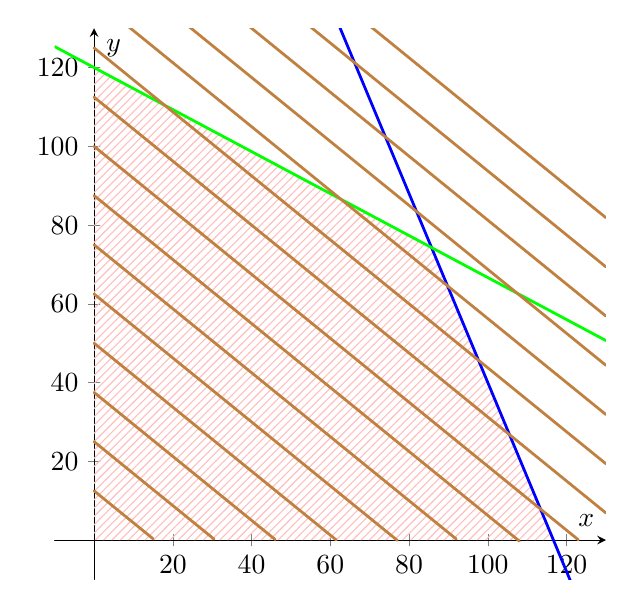
\begin{tikzpicture}[line cap=round,line join=round,>=triangle 45,x=0.1cm,y=0.1cm]
  \begin{axis}[x=0.05cm,y=0.05cm,
               axis lines=middle,
               ymajorgrids=false,
               xmajorgrids=false,
               xmin=-10,
               xmax=130,
               ymin=-10,
               ymax=130,
               xtick={-40.0,-20.0,...,300.0},
               ytick={-120.0,-100.0,...,140.0},]
   \clip(-10,-10) rectangle (130,130);
   \fill[line width=2.pt,color=pink,fill=pink,pattern=north east lines,pattern color=pink] (0.,0.) -- (116.6,0.) -- 
     (85.71428571428572,74.28571428571429) -- (0.,120.) -- cycle;
   \draw [line width=1.pt,domain=-10:130,color=blue] plot(\x,{(--70.-0.6*\x)/0.25});
   \draw [line width=1.pt,domain=-10:130,color=green] plot(\x,{(--90.-0.4*\x)/0.75});
%   \draw [line width=1.pt,color=brown,domain=0:1] plot(\x,{(-5000.-65.*\x)/80.});
%   \draw [line width=1.pt,color=brown,domain=0:130] plot(\x,{(-4000.-65.*\x)/80.});
%   \draw [line width=1.pt,color=brown,domain=0:130] plot(\x,{(-3000.-65.*\x)/80.});
%   \draw [line width=1.pt,color=brown,domain=0:130] plot(\x,{(-2000.-65.*\x)/80.});
%   \draw [line width=1.pt,color=brown,domain=0:130] plot(\x,{(-1000.-65.*\x)/80.});
%   \draw [line width=1.pt,color=brown,domain=0:130] plot(\x,{(-0.-65.*\x)/80.});
   \draw [line width=1.pt,color=brown,domain=0:15] plot(\x,{(1000.-65.*\x)/80.});
   \draw [line width=1.pt,color=brown,domain=0:30.5] plot(\x,{(--2000.-65.*\x)/80.});
   \draw [line width=1.pt,color=brown,domain=0:46] plot(\x,{(--3000.-65.*\x)/80.});
   \draw [line width=1.pt,color=brown,domain=0:61.5] plot(\x,{(--4000.-65.*\x)/80.});
   \draw [line width=1.pt,color=brown,domain=0:77] plot(\x,{(--5000.-65.*\x)/80.});
   \draw [line width=1.pt,color=brown,domain=0:92] plot(\x,{(--6000.-65.*\x)/80.});
   \draw [line width=1.pt,color=brown,domain=0:108] plot(\x,{(--7000.-65.*\x)/80.});
   \draw [line width=1.pt,color=brown,domain=0:123] plot(\x,{(--8000.-65.*\x)/80.});
   \draw [line width=1.pt,color=brown,domain=0:130] plot(\x,{(--9000.-65.*\x)/80.});
   \draw [line width=1.pt,color=brown,domain=0:130] plot(\x,{(--10000.-65.*\x)/80.});
   \draw [line width=1.pt,color=brown,domain=0:130] plot(\x,{(--11000.-65.*\x)/80.});
   \draw [line width=1.pt,color=brown,domain=0:130] plot(\x,{(--12000.-65.*\x)/80.});
   \draw [line width=1.pt,color=brown,domain=0:130] plot(\x,{(--13000.-65.*\x)/80.});
   \draw [line width=1.pt,color=brown,domain=0:130] plot(\x,{(--14000.-65.*\x)/80.});
   \draw [line width=1.pt,color=brown,domain=0:130] plot(\x,{(--15000.-65.*\x)/80.});
\draw (125,5) -- node{$x$}(125,5);
\draw (5,125) -- node{$y$}(5,125);
  \end{axis}
 \end{tikzpicture}
\end{document}